\section{\uppercase{Background}}
\label{sec:background}
\noindent

\subsection{Spurious Regression}

Regression analysis is widely used to test economic theories. But sometimes
regression is done between two variables, lets say $x_t$ and $y_t$, which are
not causally related. This occurs at the presence of a third stochastic variable
$z_t$ which is the true causal of the first two variables $x_t$ and $y_t$. The
regression measure R-squared gives high values in presence of spurious
relationships. This measure would means that the model explains all the
variability of the response data around its mean which is not true. 

The R-squared measure is calculated as follows:

\begin{equation}
\label{eq:rsquared}
R^2 = 1 - \frac{\sum_{t=1}^T \epsilon_t^2}{\sum_{t=1}^T(y_t - \bar{y})^2}
\end{equation}

In presence of spurious relationships the denominator of equation
\ref{eq:rsquared} becomes very large because a large weight is placed on extreme
observations on either side of the mean $\bar{y}$.
In order to detect this, other statistic must be considered such as the
Durbin-Watson statistic.

% Acá agregar gráfico de spurious regression

\subsection{Integration and Cointegration}
A time series $\mathbf{y}$ is said to be integrated of order $d$ if after
differentiating the variable $d$ times, we get an I(0) process, more precisely:

\[
(1-L)^d \mathbf{y} \sim \text{I(0)} \, ,
\]

\noindent where I(0) is a stationary time series and $L$ is the lag operator:

\[
(1-L)\mathbf{y} = \Delta \mathbf{y}=\mathbf{y}_t  -\mathbf{y}_{t-1} \quad \forall t
\]

Let $\mathbf{y}_t = \{\mathbf{y}^1, \dots, \mathbf{y}^l\}$ be a set of $l$
stationary time series I(1) which are said to be cointegrated if a vector
$\beta=[\beta(1),\dots,\beta(l)]^\top \in \mathbb{R}^l$  exists such that the
time series,

\begin{equation}
 \mathbf{Z}_t:= \beta^\top \mathbf{y}_t = \beta(1) \mathbf{y}^1 + \dots + \beta(l) \mathbf{y}^l \sim
 \text{I(0)}\, .
\end{equation}

In other words, a set of I(1) variables is said to be cointegrated if
a linear combination of them exists which is I(0).


\subsection{Vector Autorregresive Models}\label{sec:varvec}

VECM is a special case of VAR model and both describe the joint behaviour of a
set of variables.

VAR($p$) model is a general framework to describe the behaviour of a set of $l$
endogenous variables as a linear combination of their last $p$ values. These
$l$ variables at time $t$ are represented by the vector $\mathbf{y}_t$ as
follows:

\begin{equation}
\label{eq:variables}
\mathbf{y}_t = 
\begin{bmatrix} y_{1,t} &
y_{2,t} &
\dots &
y_{l,t}
\end{bmatrix}^\top \, ,
\end{equation}
\noindent where $y_{j,t}$ corresponds to the time series $j$ evaluated at
time $t$.

The VAR(p) model describes the behaviour of a dependent variable in terms
of its own lagged values and the lags of the others variables in the
system. The model with $p$ lags is formulated as the following:

\begin{equation}
\label{eq:var}
 \mathbf{y}_t = \phi_1 \mathbf{y}_{t-1}  + \dots +   \phi_p\mathbf{y}_{t-p}
+ \mathbf{c} + \mathbf{\epsilon}_t \, ,
\end{equation}

\noindent where $t=p+1, \dots N$,  ${\phi_1,\dots,\phi_p}$ are $l \times l$
matrices of real coefficients,
$\mathbf{\epsilon}_{p+1},\dots,\mathbf{\epsilon}_N$ are error terms,
$\mathbf{c}$ is a constant vector and $N$ is the total number of samples.

The VAR matrix form of equation~(\ref{eq:var}) is:

%\begin{equation}\label{eq:vareq}
%\mathbf{B} = \mathbf{A} \mathbf{X} + 
%\mathbf{E} \, , 
%\end{equation}
%
%\noindent where:
%\begin{eqnarray}
%\mathbf{A} &=&
%\begin{bmatrix}
%   \mathbf{y}_{p}     & \dots    & \mathbf{y}_{N-1}\\
%   \mathbf{y}_{p-1}   & \dots    & \mathbf{y}_{N-2}\\
%   \vdots             & \ddots   & \vdots\\
%   \mathbf{y}_{1}     & \dots    & \mathbf{y}_{N-p}\\
%   1                  & \dots    & 1 
%   \end{bmatrix}^\top \, ,\\
%\mathbf{B} &=&
%\begin{bmatrix}
%\quad \\
%\mathbf{y}_{p+1} &
%\dots & 
%\mathbf{y}_N \\
%\quad
%\end{bmatrix}^\top  \, ,\\
%\mathbf{X}&=&
%\left[
%\begin{array}{ccccc}
%    \quad  & \quad & \quad & \quad \\
%    \phi_1   & \cdots & \phi_p & \mathbf{c} \\  
%    \quad & \quad & \quad & \quad
%    \end{array}
%\right]^\top \, ,\\
%\mathbf{E} &=& 
%\begin{bmatrix}
%    \quad \\
%    \mathbf{\epsilon}_{p+1}  & 
%    \dots                & 
%    \mathbf{\epsilon}_N \\
%    \quad
%\end{bmatrix}^\top \, . 
%\end{eqnarray}

\begin{equation}
 \label{eq:vareq}
               \underbrace{ \begin{bmatrix}
               \quad \\
               \mathbf{y}_{p+1} &
               \mathbf{y}_{p+2} &
               \dots & 
               \mathbf{y}_N \\
               \quad
               \end{bmatrix}}_{\substack{ \mathbf{B}^\top\\l \times (N-p)}}   
= 
                \underbrace{\left[ 
                \begin{array}{ccccc}
                \quad & \quad & \quad & \quad & \quad \\
                \phi_1  & \phi_2 & \cdots & \phi_p & \mathbf{c} \\  
                \quad &\quad & \quad & \quad & \quad
               \end{array} 
               \right]}_{\substack{ \mathbf{X}^\top\\ l \times (l \times p + 1 )}}
\underbrace{\begin{bmatrix}
   \mathbf{y}_{p}  & \mathbf{y}_{p+1} & \dots    & \mathbf{y}_{N-1}\\
   \mathbf{y}_{p-1}  & \mathbf{y}_{p} & \dots    & \mathbf{y}_{N-2}\\
   \vdots        & \vdots   & \ddots   & \vdots\\
   \mathbf{y}_{1} & \mathbf{y}_{2}   & \dots    & \mathbf{y}_{N-p}\\
   1 & 1   & \dots    & 1 
   \end{bmatrix}}_{\substack{ \mathbf{A}^\top\\ (l\times p +1 )\times (N-p)}}
+
\underbrace{\begin{bmatrix}
                \quad \\
              \mathbf{\epsilon}_{p+1}  & 
              \mathbf{\epsilon}_{p+2}  & 
              \dots                & 
              \mathbf{\epsilon}_N \\
              \quad
             \end{bmatrix}}_{\substack{\mathbf{E}^\top\\l \times (N-p) }} 
\end{equation}
Equation~(\ref{eq:vareq})  can be solved using ordinary least squares estimation.

\subsection{Vector Error Correction}

VECM is a special form of a VAR model for I(1) variables that are also
cointegrated~\cite{banerjee1993}. It is obtained by replacing the form $\Delta
\mathbf{y}_t = \mathbf{y}_t - \mathbf{y}_{t-1}$ in equation (\ref{eq:var}).
VECM is expressed in terms of differences, has an error correction term and 
the following form:

\begin{equation}
 \label{eq:vec}
 \Delta \mathbf{y}_t = 
 \underbrace{ \Omega\mathbf{y}_{t-1}}_\text{Error correction term} + 
 \sum_{i=1}^{p-1}
\phi_i^* \Delta \mathbf{y}_{t-i}  + \mathbf{c} + \mathbf{\epsilon}_t \quad ,
\end{equation}

\noindent where coefficients matrices $\Omega$ and $\phi_i^*$ are
function of matrices $\phi_i$ (shown in equation (\ref{eq:var})) as follows:

\begin{eqnarray*}
\phi_i^* &: =& -\sum_{j=i+1}^{p} \phi_j \\
\Omega &: =& -(\mathbb{I}-\phi_1-\dots-\phi_p) 
\end{eqnarray*}

The matrix $\Omega$ has the following properties~\cite{johansen1995}:
\begin{itemize}
\item If $\Omega = 0$ there is no cointegration
\item If $rank(\Omega)=l$ i.e full rank, then the time series are not
I(1) but stationary
\item If $rank(\Omega)=r,\quad 0 < r < l$ then, there is cointegration
and the matrix $\Omega$ can be expressed as $\Omega =
\alpha \beta^\top$, where $\alpha$ and $\beta$ are $(l \times r)$
matrices and $rank(\alpha)=rank(\beta)=r$.

The columns of $\beta$ contains the cointegration vectors and the rows of
$\alpha$ correspond with the adjusted vectors. $\beta$ is obtained by Johansen
procedure~\cite{johansen1988} whereas $\alpha$ has to be determined as a
variable in the VECM.

It is worth noticing that the factorization of the matrix $\Omega$ is not
unique since for any $r \times r$ nonsingular matrix $H$ we have:

\begin{eqnarray*}
\alpha \beta^\top &=& \alpha \mathbf{HH^{-1}} \beta^\top\\
&=&(\alpha\mathbf{H})(\beta(\mathbf{H}^{-1})^\top)^\top \\
&=& \alpha^*(\beta^*)^\top
\end{eqnarray*}

\noindent whith $\alpha^* = \alpha\mathbf{H}$ and $\beta^* =
\beta(\mathbf{H}^{-1})^\top$.


\end{itemize}

If cointegration exists, then equation (\ref{eq:vec}) can be written as follows:


\begin{equation}
 \label{eq:vecfull}
 \Delta \mathbf{y}_t = \alpha \beta^\top\mathbf{y}_{t-1} 
 + \sum_{i=1}^{p-1} \phi_i^*\Delta
\mathbf{y}_{t-i}  + \mathbf{c} + \mathbf{\epsilon}_t \quad ,
\end{equation}

\noindent which is a VAR model but for time series differences.

VECM matricial form is the following:

%\begin{eqnarray}\label{eq:vecmatrix}
% \mathbf{A}&=&
%   \begin{bmatrix} 
%   \beta^\top \mathbf{y}_{p} & 
%   \cdots & \beta^\top \mathbf{y}_{N-1} \\
%   \Delta \mathbf{y}_p  & \cdots 
%   &\Delta\mathbf{y}_{N-1} \\ 
%   \vdots  & \ddots & \vdots \\
%   \Delta\mathbf{y}_2  & \cdots 
%   & \Delta \mathbf{y}_{N-p+1} \\
%   1 & \cdots & 1 
%   \end{bmatrix}^\top \label{eq:vecA} \, ,\\
%\mathbf{B} & = &
% \begin{bmatrix}
% \quad\\
%  \Delta \mathbf{y}_{p+1} & 
%  \dots &
%  \Delta \mathbf{y}_N \label{eq:vecB}\\
%  \quad
% \end{bmatrix}^\top \, ,\\
%\mathbf{X}&=&
%  \begin{bmatrix}
%   \quad \\
%   \alpha & \phi_1^* & \cdots & \phi_{p-1}^* & \mathbf{c} \\  
%   \quad
%   \end{bmatrix}^\top \, ,\\
%\mathbf{E} &=&
%\begin{bmatrix}
%   \quad \\
%   \mathbf{\epsilon}_{p+1} &
%   \dots &
%   \quad &\mathbf{\epsilon}_N \, \\ \quad
%\end{bmatrix}^\top 
%\end{eqnarray}
%


\begin{equation} \label{eq:vecmatrix}
\underbrace{
               \begin{bmatrix}
               \quad\\
                \mathbf{\Delta y}_{p+1} & 
                \dots &
                \mathbf{\Delta y}_N \\
                \quad
               \end{bmatrix}
               }_{\substack{\mathbf{B}^\top\\ l \times (N-p) }} =
   \underbrace{
    \begin{bmatrix}
     \quad \\
     \alpha & \phi_1^* & \cdots & \phi_{p-1}^* & \mathbf{c} \\  
     \quad
     \end{bmatrix} 
     }_{\substack{ \mathbf{X}^\top\\ l \times (l\times p +1)}}
\underbrace{\begin{bmatrix} 
   \beta^\top \mathbf{y}_{p} & 
   \cdots & \beta^\top \mathbf{y}_{N-1} \\
   \mathbf{\Delta y}_p  & \cdots 
   & \mathbf{\Delta y}_{N-1} \\ 
   \vdots  & \ddots & \vdots \\
   \mathbf{\Delta y}_2  & \cdots 
   & \mathbf{\Delta y}_{N-p+1} \\
   1 & \cdots & 1 
   \end{bmatrix}}_{\substack{\mathbf{A}^\top \\ (l \times p +1) \times (N-p) }}
+
\underbrace{\begin{bmatrix}
              \quad \\
              \mathbf{\epsilon}_{p+1} &
              \dots &
              \quad &\mathbf{\epsilon}_N \\ \quad
             \end{bmatrix}}_{\substack{\mathbf{E}^\top\\ l \times (N-p) }} 
\end{equation}

VAR and VECM parameters shown in equations (\ref{eq:vareq},\ref{eq:vecmatrix}) can be solved
using standard regression techniques, such as ordinary least squares (OLS).

\subsection{Unit Root Tests}
In order to use VECM the time series are required to be I(1) which is detected
using a unit root test. The Dickey-Fuller (ADF) test ~\cite{dickey1979} is a
unit root test where the null hypothesis is that the
variable has a unit root.

If we have a variable with the form:
\[
\mathbf{x}_t = \alpha \mathbf{x}_{t-1} + \epsilon_t
\]

\noindent and if we substract $\mathbf{x}_{t-1}$ from both sides we get:

\begin{equation}
\label{eq:DF}
\Delta \mathbf{x}_t = (\alpha-1) \mathbf{x}_{t-1} + \epsilon_t
\end{equation}

Dickey fuller test consist on determine if $\alpha$ equals 1. The alternative
hypothesis is $\alpha < 1$ which means that $\mathbf{x}_t$ is a stationary
process. 

In order to include more than 1 lagged variable the Augmented Dickey-Fuller
test was developed and their tabulated critical values were obtained
by~\cite{mackinnon2010}. The number of lags is often selected using Schwartz
criterion.

\subsection {Cointegration Tests}

Johansen method~\cite{johansen1988} allows to find cointegration among several
I(1) time series. This test is more general than the
Engle-Granger~\cite{engle1987} test which only allow to find cointegration
between two time series.  Johansen procedure takes the form of a
likelihood-ratio test which determines $r$ cointegration relationships. The
method provides two tests based on an eigenvector decomposition of the matrix
$\Omega = \alpha \beta^\top$ on equation~\ref{eq:vec} called trace and maximal
eigenvalue statistic.  Once the number of cointegration number is determined,
$r$ more significative eigenvectors provided by Johansen procedure are used to
get the cointegration vector matrix $\beta^\top$.  Critical values for both
tests are limited to 12 and 5 variables in the trace and maximal eigenvalue
statistic respectively.

The trace test null hypothesis is $H_0: r = r_0$ against $H_1: r > r_0$ and the
maximum eigenvalue test null hypothesis is $H_0: r = r_0$ against $H_1: r =
r_0+1$ starting with $r_0 = 0$.  In the latest test, if we start with $r_0=0$
and $H_0$ is rejected $H_1: r = 1$ will be accepted which is not true if there
are more than one cointegration relationship, this is why this test is less
powerful and the trace test is commonly used.







\subsection{Ordinary Least Squares method}

When $\mathbf{A}$ is singular, solution to equation~(\ref{eq:vecmatrix}) is given
by the ordinary least squares (OLS) method. OLS consists of minimizing the sum
of squared errors or equivalently minimizing the following expression:

\begin{equation}
\label{eq:regressionproblem}
\underset{\mathbf{X}}{\text{min}} \quad \| \mathbf{A}\mathbf{\mathbf{X}} - \mathbf{B} \|_2^2
\end{equation}

\noindent for which the solution $\hat{\mathbf{X}}$ is well-known:

\begin{equation}
\label{eq:MP}
\hat{\mathbf{X}}=\mathbf{A}^{\!\!+}\,\mathbf{B}
\end{equation}

\noindent where $\mathbf{A}^{\!\!+}$ is the Moore-Penrose pseudo-inverse
which can be written as follows: 

\begin{equation}
\label{eq:pseudoinverse}
\mathbf{A}^{\!\!+}= (\mathbf{A}^{\!\!\top} \mathbf{A})^{-1}\mathbf{A}^{\!\!\top} \, .
\end{equation}

However, when $\mathbf{A}$ is not full rank, i.e
$rank(\mathbf{A})=k <  n \leq m$, $\mathbf{A}^\top \mathbf{A}$ is
always singular and equation~(\ref{eq:pseudoinverse}) cannot be used.
More generally, the pseudo-inverse is best computed using the compact
singular value decomposition (SVD) of $\mathbf{A}$:

\begin{equation}
    \label{eq:compactsvd}
    \underset{m \times n}{\mathbf{A}}=
    \underset{m \times k}{\mathbf{U_1}} \enskip
    \underset{k \times k}{\Sigma_1} \enskip
    \underset{k \times n}{\mathbf{V}_1^{\top}} \, ,
\end{equation}

\noindent as follows

\begin{equation}
\label{eq:pseudoinversesvd}
\mathbf{A}^{\!\!+} = \mathbf{V}_1 \Sigma_1^{-1} \mathbf{U}_1^\top \, .
\end{equation}

%Descomentar en la tesis
\textbf{Demo}\quad

Since $\mathbf{A}$ is singular the problem shown in
equation~(\ref{eq:regressionproblem}) has not solution, the minimum norm given
by equation~(\ref{eq:MP}) is obtained by solving the equivalent problem:

\begin{equation*}
\label{eq:proyectorsol}
\mathbf{A \hat{X} = PB} 
\end{equation*}

\noindent where $\mathbf{P=U_1 U_1^\top}$ is the projection onto the
Col($\mathbf{A}$). 

Since $\mathbf{V} = [\underset{(n \times k)}{\mathbf{V_1}} |
\underset{(n \times k)}{\mathbf{V_2}}]$ and $\mathbf{V_1^\top V_2 =
0}$ we can express $\mathbf{\hat{X}} = \mathbf{V_1 x_1 + V_2 x_2}$
with $\mathbf{x_2=0}$ because $\mathbf{\hat{X}}$ lives in the
$\text{Row}(\mathbf{A})$ given by $\mathbf{V_1}$, so we have:

\begin{eqnarray*}
\mathbf{A \hat{X}} &=& \mathbf{PB} \\
\mathbf{U_1 \Sigma_1 V_1^\top \hat{X}} &=& \mathbf{U_1 U_1^\top B} \\
\mathbf{ V_1^\top \hat{X}} &=&  \mathbf{\Sigma_1^{-1} U_1^\top B} \\ 
\mathbf{ V_1^\top V_1 x_1} &=& \mathbf{\Sigma_1^{-1}
U_1^\top B} \\
\mathbf{x_1}&=& \mathbf{\Sigma_1^{-1} U_1^\top B}
\end{eqnarray*}

\noindent from this result we can obtain $\mathbf{\hat{X}}$ and
therefore the pseudo-inverse expression:

\begin{eqnarray*}
\mathbf{\hat{X}} &=& \mathbf{V_1 x_1} \\
                &=& \mathbf{V_1 \Sigma_1^{-1} U_1^\top B} \\
\mathbf{A^+} &=& \mathbf{V_1 \Sigma_1^{-1} U_1^\top} \, .
\end{eqnarray*}




\subsection{Ridge Regression}\label{sec:RR}

Ridge regression (RR) introduces a ridge estimation to avoid the
singularity of the matrix $\mathbf{A}^\top \mathbf{A}$
equation~(\ref{eq:pseudoinverse}). RR solves the following
optimization problem:

\begin{equation}
\label{eq:RRproblem}
\underset{\mathbf{X}}{\text{min}} \quad \|
\mathbf{A}\mathbf{\mathbf{X}} - \mathbf{B} \|_2^2 +\lambda \|
\mathbf{\mathbf{X}}\|_2^2 
\end{equation}

\noindent where $\lambda$ is a regularization parameter. 

The RR optimal solution $\mathbf{X}(\lambda)$ is also well-known: 

\begin{equation}
\label{eq:optsolRR}
\mathbf{X}(\lambda)=(\mathbf{A}^\top \mathbf{A}+ \lambda
\mathbb{I})^{-1}\mathbf{A}^\top \mathbf{B} \, . 
\end{equation}


\textbf{Demo}\quad

To solve equation~(\ref{eq:optsolRR}) is equivalent to solve the following
optimization problem:


\begin{equation}
\label{eq:RRproblem2}
\underset{\mathbf{X}(\lambda)}{\text{min}} \quad \|
\mathbf{C}\mathbf{\mathbf{X}} - \mathbf{F} \|_2^2
\end{equation}

\noindent where

\begin{equation*}
	\mathbf{C}=\begin{bmatrix} \quad &\mathbf{A}& \quad \\ \hdashline \quad
& \lambda\mathbb{I}&\quad  \end{bmatrix} \quad \text{and} \quad
	\mathbf{F}=\begin{bmatrix} \quad &\mathbf{B}& \quad \\ \hdashline \quad
& \mathbf{0}&\quad  \end{bmatrix} \, .
\end{equation*}

Applying equation~(\ref{eq:MP}) and considering that $\mathbf{C}^\top
\mathbf{C} = \mathbf{A}^\top \mathbf{A} + \lambda \mathbb{I}$ and 
$\mathbf{C}^\top \mathbf{F}=\mathbf{A}^\top \mathbf{B} $ we have:

\begin{eqnarray*}
\mathbf{X}(\lambda)&=&(\mathbf{C}^\top
\mathbf{C})^{-1}\mathbf{C}^\top \mathbf{F} \\
&=& (\mathbf{A}^\top \mathbf{A} + \lambda \mathbb{I})^{-1} \mathbf{A}^\top \mathbf{B}
\end{eqnarray*}

\subsection{Online Ridge regression}

If we represent matrices $\mathbf{A}$ and $\mathbf{B}$ such as:

\begin{equation}
\label{eq:notation}
	\mathbf{A} = 
\left[
  \begin{tabular}{c>{$}c<{$}c}
    --- & \mathbf{a}^{\top}_{1} & ---\\
    --- & \mathbf{a}^{\top}_{2} & ---\\
    & \vdots & \\
    --- & \mathbf{a}^{\top}_{m} & ---
  \end{tabular}
\right]
\quad \text{and} \quad
\mathbf{B} =
\left[
  \begin{tabular}{c>{$}c<{$}c}
    --- & \mathbf{b}_{1} & ---\\
    --- & \mathbf{b}_{2} & ---\\
    & \vdots & \\
    --- & \mathbf{b}_{m} & ---
  \end{tabular}
\right] \, ,
\
\end{equation}

\noindent equation~(\ref{eq:optsolRR}) can also be written as:

\begin{eqnarray*}
\label{eq:RReapand}
\mathbf{\mathbf{X}}_{\text{ridge}}&=&(\mathbf{A}^\top \mathbf{A}+ \lambda
\mathbb{I})^{-1}\mathbf{A}^\top \mathbf{B} \\
&=& \displaystyle \big (\sum_{t=1}^m
\mathbf{a}_t \mathbf{a}_t  ^\top + \lambda \mathbb{I}\big )^{-1}
\sum_{t=1}^m \mathbf{a}_t \mathbf{b}_t \, .
\end{eqnarray*}

Lets define $\displaystyle\mathbf{S}= \sum_{t=1}^m \mathbf{a}_t
\mathbf{a}_t  ^\top + \lambda \mathbb{I} $ and $\mathbf{W}=
\displaystyle\sum_{t=1}^m \mathbf{a}_t \mathbf{b}_t$, so the
algorithm~\ref{alg:RR} shows the iterative formulation:

\begin{algorithm}[H]
\begin{algorithmic}[1]
\REQUIRE $\,$ \\
$\{\mathbf{a}_1,\dots,\mathbf{a}_{m} \}$: $m$ input vectors \\
$\{\mathbf{b}_1,\dots,\mathbf{b}_{m} \}$: $m$ target vectors \\
$\lambda$: regularization parameter \\
\ENSURE  $\,$ \\
$\{f(\mathbf{a}_1),\dots,f(\mathbf{a}_{m}) \}$: model predictions \\
\STATE Initialize $\mathbf{S}=\lambda \mathbb{I}$
and $\mathbf{W}=0$
\FOR { $t = 1$ to $m$ }
	\STATE read new $\mathbf{a}_t$
	\STATE $\mathbf{X}=\mathbf{S}^{-1}\mathbf{W}$
	\STATE output prediction $f(\mathbf{a}_t) = \mathbf{X}^\top \mathbf{a}_t$
   	\STATE $\mathbf{S} = \mathbf{S} + \mathbf{a}_t \mathbf{a}_t^\top$
   	\STATE Read new $y_t$
    	\STATE $\mathbf{W} = \mathbf{W} + \mathbf{a}_t \mathbf{b}_t$
\ENDFOR
\end{algorithmic}
\caption{Online Ridge Regression}
\label{alg:RR}
\end{algorithm}



\subsection{The Aggregating Algorithm for Regression}

The AAR, proposed by~\cite{vovk2001}, is an application of the aggregating
algorithm to the problem of regression. The idea is to introduce the new input
vector $\mathbf{x}_{m+1}$ to solve the model parameters: 

\begin{equation}
\label{eq:AARexpand}
\mathbf{X}_{aar} = \displaystyle \big (\sum_{t=1}^{m+1}
\mathbf{a}_t \mathbf{a}_t  ^\intercal + \gamma \mathbb{I}\big )^{-1}
\sum_{t=1}^m \mathbf{a}_t \mathbf{b}_t \, .
\end{equation}

If we define $\displaystyle\mathbf{S}= \sum_{t=1}^{m+1} \mathbf{a}_t
\mathbf{a}_t  ^\intercal + \gamma \mathbb{I} $ and $\mathbf{W}=
\displaystyle\sum_{t=1}^m \mathbf{a}_t \mathbf{b}_t$, the
algorithm~\ref{alg:AAR} is slightly different to the algorithm~\ref{alg:RR}, 
which updated matrix $\mathbf{S}$ before making the prediction:

\begin{algorithm}[ht]
\begin{algorithmic}[1]
\REQUIRE $\,$ \\
$\{\mathbf{a}_1,\dots,\mathbf{a}_{m} \}$: $m$ input vectors \\
$\{\mathbf{b}_1,\dots,\mathbf{b}_{m} \}$: $m$ target vectors \\
$\lambda$: regularization parameter \\
\ENSURE  $\,$ \\
$\{f(\mathbf{a}_1),\dots,f(\mathbf{a}_{m}) \}$: model predictions \\
\STATE Initialize $\mathbf{S}=\lambda \mathbb{I}$
and $\mathbf{W}=0$
\FOR { $t = 1$ to $m$ }
	\STATE read new $\mathbf{a}_t$
   	\STATE $\mathbf{S} = \mathbf{S} + \mathbf{a}_t \mathbf{a}_t^\intercal$
	\STATE $\mathbf{X}=\mathbf{S}^{-1}\mathbf{W}$
	\STATE output prediction $f(\mathbf{a}_t) = \mathbf{X}^\intercal \mathbf{a}_t$
   	\STATE Read new $\mathbf{y}_t$
    	\STATE $\mathbf{W} = \mathbf{W} + \mathbf{a}_t \mathbf{b}_t$
\ENDFOR
\end{algorithmic}
\caption{{\em The aggregating algorithm for regression}}
\label{alg:AAR}
\end{algorithm}






\subsection{Selection of Lambda}

The additional term $\lambda \|\mathbf{\mathbf{X}}\|_2^2$ in the optimization
problem shown in equation~(\ref{eq:RRproblem}) has two effects on the solution:
shrinks the coefficients towards zero and improves the conditioning of the
problem.

Figure~\ref{fig:shrinks} shows a visual example of the shrinking of the
coefficients:

\begin{figure}[h!]
\includegraphics[width=0.5\linewidth]{img/shrinks}
\caption{Shrink of regression coefficients}
\label{fig:shrinks}
\end{figure}


On the other hand, the effect of adding the term $\lambda \mathbb{I}$
to the matrix $\mathbf{A}^\top \mathbf{A}$
(equation~(\ref{eq:optsolRR})) improves its condition number since it
increases its diagonal values when $\lambda > 0 $.  The matrix
$\mathbf{A}^\top \mathbf{A}$ is symmetrical ($(\mathbf{A}^\top
\mathbf{A})^\top = \mathbf{A}^\top \mathbf{A}$) and therefore
diagonalizable.  If we know the eigenvalue decomposition of $\mathbf{A}
= \mathbf{U\Sigma V^\top}$, then:

\begin{eqnarray*}
\mathbf{A}^\top \mathbf{A}+\lambda \mathbb{I}&=&\mathbf{V\Sigma^2
V}^\top + \lambda \mathbf{V} \mathbf{V}^\top\\ &=&\mathbf{V}
(\mathbf{\Sigma}^2+\lambda\mathbb{I}) \mathbf{V}^\top \, ,
\end{eqnarray*}

\noindent where

\begin{equation*}
\mathbf{\Sigma}^2+\lambda\mathbb{I}=
\begin{bmatrix}
\sigma^2_1 + \lambda & \, & \, \\
\, & \sigma^2_2 +\lambda & \, \\
\, & \, & \ddots & \, \\
\, & \, & \, & \sigma^2_n +\lambda \, .
\end{bmatrix}
\end{equation*}

where $\sigma_1 \geq \sigma_2 \geq \dots \geq \sigma_n$.

Since the condition number of a matrix $\mathbf{A}$ is defined as:

\begin{equation*}
	\kappa = \|\mathbf{A}\| \|\mathbf{A}^{-1}\|
\end{equation*}

If matrix $\mathbf{A}$ is non-singular, its condition number can be
expressed in terms of its singular values. The effect of adding the
regularization term affects the condition number as follows:

\begin{eqnarray*}
\kappa_{ols} &=& \|\mathbf{A}\| \|\mathbf{A}^{-1}\|=\frac{\sigma_1}{\sigma_n} \\
\kappa_{ridge} &=& \|\mathbf{A}^\intercal \mathbf{A} + \lambda \mathbb{I}\| 
\|(\mathbf{A}^\intercal \mathbf{A} + \lambda \mathbb{I})^{-1}\|=\frac{\sigma_1+\lambda}{\sigma_n + \lambda} \,
\end{eqnarray*}

It is easy to see that the term $\lambda$ improves the condition number: 

\begin{equation*}
        \frac{\sigma_1+\lambda}{\sigma_n + \lambda} <
        \frac{\sigma_1}{\sigma_n} \,  \qquad \forall \quad \lambda > 0
\end{equation*}


However, $\lambda$ cannot be too large. Tipically $\lambda$ is small and its
magnitude depends on the matrix $\mathbf{A}$.

For rank deficient matrices we know that $\text{det}(\mathbf{A A^\top})=0$, adding the
term $\lambda \mathbb{I}$ we have that $\text{det}(\mathbf{A A^\top}+\lambda \mathbb{I}) =
p(\lambda)$ where $p(\lambda)$ is a polynomial of degree $n$ ($\mathbf{A}$ is
$m \times n$). The zeros of $p(\lambda)$ are discretes, so it can be represented
as:

\[
p(\lambda) =
\lambda(\lambda-\lambda_1)^{n_1}(\lambda-\lambda_2)^{n_2}\dots(\lambda-\lambda_s)^{n_s}
\]

\noindent where $n_1 + n_2 + \dots + n_s = n$.

This means that $\lambda$ must be small in order to ensure that $p(\lambda)$
does not vanish.

\subsubsection{The bias-variance tradeoff}

To determine parameter $\lambda$ is crucial for ridge regression since it could
reduce the expected prediction error by reducing variance considering a biased
estimator, this is called the bias-variance trafeoff. The prediction error is
obtained as:

\begin{equation}
 \label{eq:prederror}
E[(B-\hat{f}(\mathbf{X}))^2] = \sigma^2 + Bias(\hat{f}(\mathbf{X}))^2 + Var(\hat{f}(\mathbf{X}))
\end{equation}

\noindent where $\hat{f}(\mathbf{X})=\mathbf{AX}(\lambda)$ and
$f(\mathbf{X})=\mathbf{AX}$.


\textbf{Demo}\quad

\begin{eqnarray*}
E[(B-\hat{f}(\mathbf{X}))^2] & =&
E[(B-f(\mathbf{X})+f(\mathbf{X})-\hat{f}(\mathbf{X}))^2] \\
&=& E[(B-f(\mathbf{X}))^2] +
E[(f(\mathbf{X})-\hat{f}(\mathbf{X}))^2] + \dots \\
& &
2\cancelto{0}{E[B-f(\mathbf{X})]}E[f(\mathbf{X})-\hat{f}(\mathbf{X})] \\
&=& \sigma^2 + MSE(\hat{f}(\mathbf{X}))
\end{eqnarray*}

\noindent where 

\begin{eqnarray*}
    MSE(\hat{f}(\mathbf{X})) &=&
    E[f(\mathbf{X})-\hat{f}(\mathbf{X}))]^2 \\
    &=& E[f(\mathbf{X})-E[\hat{f}(\mathbf{X})] +
    E[\hat{f}(\mathbf{X})]-\hat{f}(\mathbf{X}))]^2 \\
    &=&  E[(f(\mathbf{X})-E[\hat{f}(\mathbf{X})])^2] +
      E[(\hat{f}(\mathbf{X})-E[\hat{f}(\mathbf{X})])^2] + \dots\\
    & & E[(f(\mathbf{X})-E[\hat{f}(\mathbf{X})])] 
    \cancelto{0}{E[(\hat{f}(\mathbf{X})-E[\hat{f}(\mathbf{X})])]} \\
    &=& Bias(\hat{f}(\mathbf{X}))^2 + Var(\hat{f}(\mathbf{X}))
\end{eqnarray*}

The bias of OLS is:

\begin{eqnarray*}
Bias(\hat{\mathbf{X}}) &=& E[\hat{\mathbf{X}}] - \mathbf{X} \\
&=& E[ (\mathbf{A}^\top \mathbf{A})^{-1}\mathbf{A}^\top \mathbf{B}] - \mathbf{X} \\
&=& E[ (\mathbf{A}^\top \mathbf{A})^{-1}\mathbf{A}^\top (\mathbf{AX})] - \mathbf{X}  \\
&=& \mathbf{X}  - \mathbf{X}  \\
&=&  0
\end{eqnarray*}


The bias of ridge regression when $\mathbf{A A^\top}$ is non-singular
can be obtained expressing ridge regression solution
$\mathbf{\lambda}$ in terms of OLS solution $\hat{\mathbf{X}}$:

\begin{eqnarray*}
\mathbf{X}(\lambda) &=&( \mathbf{A}^\top \mathbf{A} + \lambda \mathbb{I})^{-1}\mathbf{B} \\
&=& (\mathbb{I} + \lambda (\mathbf{A}^\top \mathbf{A})^{-1})^{-1} (\mathbf{A}^\top \mathbf{A})^{-1}\mathbf{A}^\top \mathbf{B} \\
&=&  (\mathbb{I} + \lambda (\mathbf{A}^\top \mathbf{A})^{-1})^{-1}  \hat{\mathbf{X}} \\
&=& \mathbf{W} \hat{\mathbf{X}} 
\end{eqnarray*}

\noindent where $\mathbf{W}  = (\mathbb{I} + \lambda (\mathbf{A}^\top
\mathbf{A})^{-1})^{-1}  $ it is defined for simplicity. Ridge
regression bias is then obtained as:

\begin{eqnarray*}
Bias(\mathbf{X}(\lambda)) &=& E[\mathbf{X}(\lambda)] - \mathbf{X} \\
&=& E[\mathbf{W}\hat{\mathbf{X}}] - \mathbf{X} \\
&=&  \mathbf{W} \mathbf{X} - \mathbf{X} \neq 0 
\end{eqnarray*}



The variance of OLS is:

\begin{equation*}
Var(\hat{\mathbf{X}}) = \sigma^2 (\mathbf{A}^\top \mathbf{A} )^{-1}
\end{equation*}

\noindent and the variance of ridge regression is:

\begin{eqnarray*}
Var(\mathbf{X}(\lambda)) &=& Var(\mathbf{W}\hat{\mathbf{X}}) \\ 
&=& \mathbf{W}Var(\hat{\mathbf{X}})\mathbf{W}^\top \\
&=& \sigma^2 \mathbf{W}(\mathbf{A}^\top \mathbf{A} )^{-1}\mathbf{W}^\top
\end{eqnarray*}


\begin{figure}[h!]
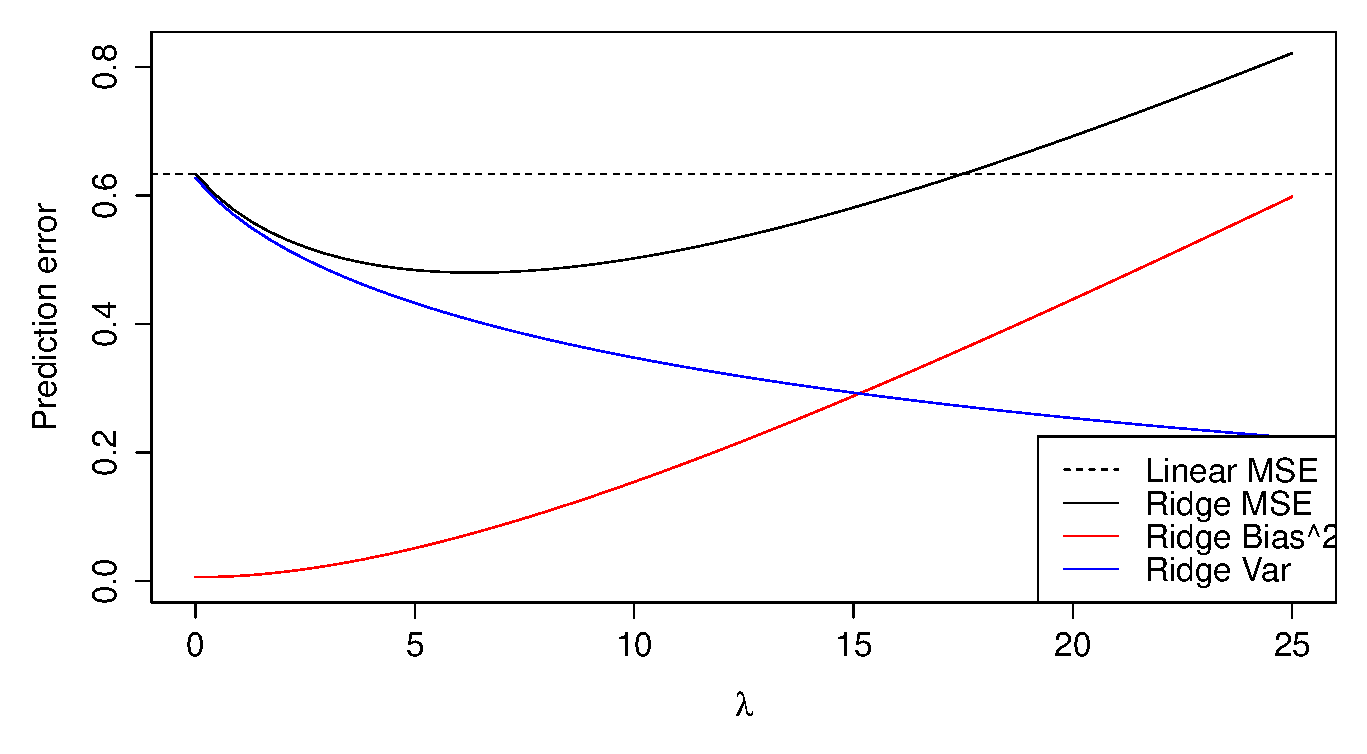
\includegraphics[width=0.8\linewidth]{img/biasvariance}
\caption{Bias-variance tradeoff}
\label{fig:biasvariance}
\end{figure}

The figure~\ref{fig:biasvariance} shows the bias-variance tradeoff
given by equation~(\ref{eq:prederror}). Ridge regression shows an
increasing bias and a decreasing variance. Despite OLS has zero bias,
its variance is greater than ridge for small values of $\lambda$.
It can be shown that, in terms of prediction error, ridge (black line)
is lower than OLS (dotted line)~\cite{hoerl1970}.



\subsubsection{Methods for lambda selection}

Despite the bias-variance tradeoff provides a conceptual framework for
determining a good model, is not directly useful. Some popular methods
for determine model selection are:

\begin{itemize}
    \item Akaike information criterion (AIC) (Akaike, 1974)
    \item Bootstrap-based selection (Efron and Tibshirani, 1997)
    \item Cross-validation (Stone, 1974)
\end{itemize}

On the other hand, $\lambda$ can also be used to reduce computational time as it
is shown in equation~(\ref{eq:taylor}). Golub (~\cite{golub1965}) suggested that
$\lambda$ had to be chosen so that:

\[
\frac{\lambda}{\lambda + \delta^2} < 0.1
\]

\noindent where $\delta$ is a lower bound of the smallest non-zero singular
value $\sigma_k$. One approach is to choose the greatest lower bound for
$\delta=\sigma_k$. Hence:

\[
\frac{\lambda}{\lambda + \sigma_k^2} < 0.1
\]

\noindent if we choose $\lambda=\beta \sigma_k^2$ then we get the following
relation:


\[
\frac{\beta \sigma_k^2}{\beta \sigma_k^2 + \sigma_k^2} =
\frac{\beta}{\beta+1} < 0.1 \Rightarrow \beta < \frac{1}{9}  
\]

Experiments done by ~\cite{coleman+sun2010} have shown that $\beta = 0.01$
produces satisfactory results. This means that $\lambda = 0.01 \sigma_k^2$.

However, get $\sigma_k$ imply obtaining first the SVD, which is
computational expensive.

Since the algorithm presented by ~\cite{coleman+sun2010} already compute the QR
factorization of the matrix $\mathbf{A}$ they show a procedure for getting
a $\lambda$ approximation using QR.

\begin{enumerate}
\item Compute QR factorization: $\mathbf{A} = \mathbf{Q_1R_1}$
\item Let $\mathbf{W}$ denote the set of absolute values of the nonzero diagonal
elements of $\mathbf{R_1}$. Let $w_{\text{min}}$ and $w_{\text{max}}$ denote the
smallest and largest elements of $\mathbf{W}$ respectively. Both 
$\lambda_1 = \hat{\beta} w_{\text{min}}^2$
$\lambda_2 = \hat{\beta} \frac{w_{\text{min}}^2}{w_{\text{max}}^2}$ where
$\hat{\beta}=0.00025$ produce satisfactory results.
\item The $\lambda_{\text{QR}}$ approximation is obtained as:
$\lambda_{\text{QR}} = \frac{\lambda_1 + \lambda_2}{2}$  
\end{enumerate}

\subsection{Efficient computation}

%Revisar!!!
In regression problems we always require getting a matrix inverse which is
computationally expensive. However, in stream data problems the is a way to
obtain a matrix inverse approximation using the Sherman-Morrison-Woodbury. This
formula allows to get the inverse of a
the matrix $\mathbf{A+uv^\top}$ if we already calculated the
inverse of $\mathbf{A}$ as follows:

\begin{equation}
\label{eq:SMW}
(\mathbf{A+uv^\top})^{-1}=\mathbf{A}^{-1}-
\frac{\mathbf{A^{-1}uv^\top A^{-1}}}{\mathbf{1+v^\top A^{-1}u}}
\end{equation}

%Revisar!!

Another way was presented by Coleman and
Sun~\cite{coleman+sun2010} using an iterative algorithm which
uses $\mathbf{X}(\lambda)$ to approximate $\mathbf{X}(0)$.


Using the compact SVD (shown in equation~(\ref{eq:compactsvd}))
$\mathbf{X}(\lambda)$ is expressed as follows:


\begin{eqnarray}
\label{eq:optsolRRsvd}
\mathbf{X}(\lambda) & = & (\mathbf{A}^\top \mathbf{A}+ \lambda
\mathbb{I})^{-1}\mathbf{A}^\top \mathbf{B} \nonumber \\
& = &\mathbf{V}_1(\Sigma_1^2+\lambda \mathbb{I})^{-1}\mathbf{\Sigma_1
U_1^\top B}
\end{eqnarray}

\noindent where is easy to see that $\mathbf{X}(\lambda) \rightarrow
\mathbf{\hat{X}}=\mathbf{V}_1 \mathbf{\Sigma}_1^{-1}\mathbf{U}_1^\top
\mathbf{B}$ as $\lambda \rightarrow 0$. 

The method consists in obtaining $\mathbf{X}(\lambda)$ and then refine
by adding more terms of its Taylor expansion to approximate
$\mathbf{X}(0) = \mathbf{\hat{X}}$. The Taylor expansion about $\lambda_0$ is:

\begin{equation}
\label{eq:taylor}
    \mathbf{X}(\lambda)=\mathbf{X}(\lambda_0) + \sum_{k=1}^\infty
    \mathbf{s}_k(\lambda-\lambda_0)^{k}
\end{equation}


\noindent where $\mathbf{s}_k=\frac{1}{k!}\mathbf{X}(\lambda)^{(k)}$
and $\mathbf{X}(\lambda)^{(k)}$ is obtained by taking differences 
$\frac{\partial}{\partial \lambda}$ of:  

\begin{eqnarray*}
(\mathbf{A}^\top \mathbf{A}+ \lambda\mathbb{I}) \mathbf{X}(\lambda) & = & \mathbf{A}^\top \mathbf{B}\\
(\mathbf{A}^\top \mathbf{A}+ \lambda\mathbb{I}) \mathbf{X}(\lambda)^{(1)} + \mathbf{X}(\lambda)& = & 0 \\
\mathbf{X}(\lambda)^{(1)}  &=& -(\mathbf{A}^\top \mathbf{A}+ \lambda\mathbb{I}) ^{-1} \mathbf{X}(\lambda) \\
\mathbf{X}(\lambda)^{(2)}  &=& -2(\mathbf{A}^\top \mathbf{A}+ \lambda\mathbb{I}) ^{-1} \mathbf{X}(\lambda)^{(1)} \\
& \vdots & \\
\mathbf{X}(\lambda)^{(k)}  &=& -k(\mathbf{A}^\top \mathbf{A}+ \lambda\mathbb{I}) ^{-1} \mathbf{X}(\lambda)^{(k-1)} 
\end{eqnarray*}



\noindent for $\lambda=0$ we have:

\begin{equation}
\label{eq:taylor}
    \mathbf{X}(0)=\mathbf{X}(\lambda_0) + \sum_{k=1}^\infty
     (-1)^k \mathbf{s}_k \lambda_0^k
\end{equation}


\noindent therefore in order to ensure convergence, we can see that$\lambda_0$
selection cannot be large. 

The algorithm for computing $\mathbf{X}(0)$ is the following:

\begin{algorithm}[H]
\begin{algorithmic}[1]
\REQUIRE $\,$ \\
$\mathbf{A}$: design matrix \\
$\mathbf{B}$: response matrix \\
$\lambda$: rank deficient parameter \\
\ENSURE  $\,$ \\
$\mathbf{X}$: parameters \\
\STATE $\mathbf{M}=\mathbf{A^\top A}$ \\
\STATE Initialize $\mathbf{Q R}=\mathbf{M}$ \\
\STATE $\mathbf{X} = \mathbf{R^{-1}Q^\top B}$ \\
\STATE $\mathbf{s} = \mathbf{X}$ \\
\FOR { $i = 1,2,3,\dots$ }
	\STATE $\mathbf{s} =
        -(\mathbf{M}+\lambda\mathbb{I})^{-1}\mathbf{s}$\\
	\STATE $\mathbf{X}=\mathbf{X} + (-1)^i {\color{red}\mathbf{s}
        \lambda^i}$
\ENDFOR
\end{algorithmic}
\caption{Algorithm for handling rank deficient matrices}
\label{alg:coleman}
\end{algorithm}

The algorithm~\ref{alg:coleman} solves equation~(\ref{eq:taylor}). However, this
version is unstable since tipically $\|\mathbf{s}\|$ is very large and
$\lambda^i$ is very small ($\lambda$ is small).

The following algorithm shows a more stable version of
algorithm~\ref{alg:coleman}.


\begin{algorithm}[H]
\begin{algorithmic}[1]
\REQUIRE $\,$ \\
$\mathbf{A}$: design matrix \\
$\mathbf{B}$: response matrix \\
$\lambda$: rank deficient parameter \\
\ENSURE  $\,$ \\
$\mathbf{X}$: parameters \\
\STATE $\mathbf{M}=\mathbf{A^\top A}$ \\
\STATE Initialize $\mathbf{Q R}=\mathbf{M}$ \\
\STATE $\mathbf{X} = \mathbf{R^{-1}Q^\top B}$ \\
\STATE $\mathbf{t} = \mathbf{X}$ \\
\FOR { $i = 1,2,3,\dots$ }
        \STATE $\mathbf{t} =\lambda \mathbf{t}$  
        \STATE $\mathbf{t} =  -(\mathbf{M}+\lambda\mathbb{I})^{-1}\mathbf{t}$
	\STATE $\mathbf{X}=\mathbf{X} + \mathbf{t}$
\ENDFOR
\end{algorithmic}
\caption{Algorithm for handling rank deficient matrices improved}
\label{alg:colemanimproved}
\end{algorithm}

Both algorithms are equivalent, but algorithm~\ref{alg:colemanimproved} is more
stable and converges in tipically less than 10 steps.
It is important to notice that the QR factorization is computed only once and it
is computationally less expensive than the SVD.

\subsection{Online machine learning algorithms}

An online algorithm allows incremental learning by processing one instance at a
time. This is done updating the current model instead of building the model from
scratch.

Training phase is commonly a computationally expensive process. Therefore, when
new data arrives it can't be included easily to the model. Moreover, it could
happen that we won't have enought time to process the new data before more data
arrives. In online learning algorithms there is no training phase, but the model
is updated and evaluated at every time step. This model updating is
computationally less expensive than a training phase.

Online learning is specially useful for stream data problems and the model is
sensitive to new data. It is also useful when some past data may be irrelevant
or we want to improve computational efficiency. However, online algorithms could
affect accuracy.

There are several popular online methods such as
perceptron~\cite{rosenblatt58},winnow~\cite{littlestone1988},
passive-aggressive~\cite{crammerETall2006}, stochastic gradient
descent~\cite{zhang2004}, aggregating algorithm~\cite{vovk2001} and the second
order perceptron~\cite{cesa-bianchi2005}.  In \cite{blum1998} and
\cite{cesa-bianchi2006} an in-deph analysis of online learning is provided.
Applications in finance has been widely used: study presented
by~\cite{arce+salinas2012} applied ridge regression in an online context and
more recently, time series forecasting using online learning has been
presented~\cite{anavaetAl2013}.

Incremental learning refers to any online learning process that learns the same
model as would be learnt by a batch learning algorithm. 

Incremental learning is useful when the input to a learning process is stream
data, with the need or desire to be able to use the result of learning at any
point in time, based on the input observations received so far. 

In principle, the stream of observations may be infinitely long, or the next
observation long delayed, precluding any hope of waiting until all the
observations have been received. One would rather not simply accumulate and
store all the inputs and, upon receipt of each new one, apply a batch learning
algorithm to the entire sequence of inputs received so far. It would be
preferable compu- tationally if the existing hypothesis or other artifact of
learning could be updated in response to each newly received input observation.

Incremental learning is very useful when there is no need to record fundamental
data and only a summary needs to be retained. Due to this, incremental
algorithms are often characterized as memoryless, because no memory of past data
is required.  The algorithm is online but not incremental if it doesn't produce
the same result for all observations that the corresponding batch algorithm
would for these same observations.

Algorithm~\ref{alg:onlinealg} shows the online learning algorithm structure:

\begin{algorithm}[ht]
\begin{algorithmic}[1]
    \STATE Receives input $\mathbf{x}_t$
    \STATE Makes prediction $\mathbf{\hat{y}}_t$
    \STATE Receives response $\mathbf{y}_t$
    \STATE Incurs loss $l_t(\mathbf{y}_t,\mathbf{\hat{y}}_t)$
\end{algorithmic}
\caption{Structure of a Learning System}
\label{alg:onlinealg}
\end{algorithm}

\noindent where $l$ is some loss function. Performance is later measured after
$T$ trials as:

\begin{equation*}
L_T = \sum_{t=1}^T l_t(\mathbf{y}_t,\mathbf{\hat{y}}_t)
\end{equation*}

The objective is minimize this loss function for all instances.
The quality of online learning algorithms is measured by a quantity known as
regret which is the difference between the performance of the online algorithm
and its optimal predictor $E^* \in \Theta$ given by:

\begin{equation*}
L^*_T= \text{min}_{E \in \Theta} L_T^E \, ,
\end{equation*}

\noindent where $L_T^E = \sum_{t=1}^T
l_t(\mathbf{y}_t,\mathbf{y}^E_t)$ and $\mathbf{y}^E_t$ is the expert estimation. 

Therefore regret is defined as:

\begin{equation*}
R_T = L_T - L^*_T
\end{equation*}


%An online learning algorithm looks at every example exactly once.
\subsection{Model selection}
In order to set model parameters the Akaike Information Criterion (AIC) is
used. AIC is often used in model selection where AIC whith smaller values are
preferred.

AIC is calculated as follows:

\begin{equation}
\label{eq:aicformula}
AIC = \underset{\text{bias}}{-\frac{2l}{N}} + 
\underset{\text{variance}}{\frac{2k}{N}}
\end{equation}

\noindent where 

\begin{description}
\item[l] is the loglikelihood function
\item[k] number of estimated parameters (including the variance)
\item[N] number of observations
\end{description}


